\chapter{Server communication}
This chapter describes the communication between server and client, aswell as the design choices and
implementation of database. \todo{Bør database være et kapitel for sig selv?}

\section{Communication}
\label{sec:com}

The communication betweeen the client application and the server is done by HTTP POST requests.
The client sends a HTTP POST request to the server containing a certain list of parameters which
define what the server is supposed to do. All requests must take atleast two required parameters, a \textit{RequestCode} and a
\textit{Type}.

\textit{RequestCode} is an integer that is simply passed through the server, it is not handled in any
way on the server. The purpose of the RequestCode parameter is to distinguish the request on the client allowing
it to execute the related function.

\textit{Type} is used to identify the request. A typical request is to get a list of feeds, and the
value of the \textit{Type} parameter would be ``GetFeeds'' in this case.

Depending on the \textit{Type} of the request, additional parameters may be required.\\

\textit{GetFeeds} takes the following parameters: \todo{bør jeg nævne alle de forskellige requests?
  eller kun eksempler?}
\begin{itemize}
\item RequestCode
\item UserId
\item Limit
\end{itemize}

\section{Database}
We are using a MySQL database with the MyISAM storage engine and which is located at a remote server. \todo{info om hvor osv.?}

The server is to contain all data about each exhibition, the companies at the exhibition, the feeds, the schedule, and some basic information about the users.

\begin{figure}[H]
\centering
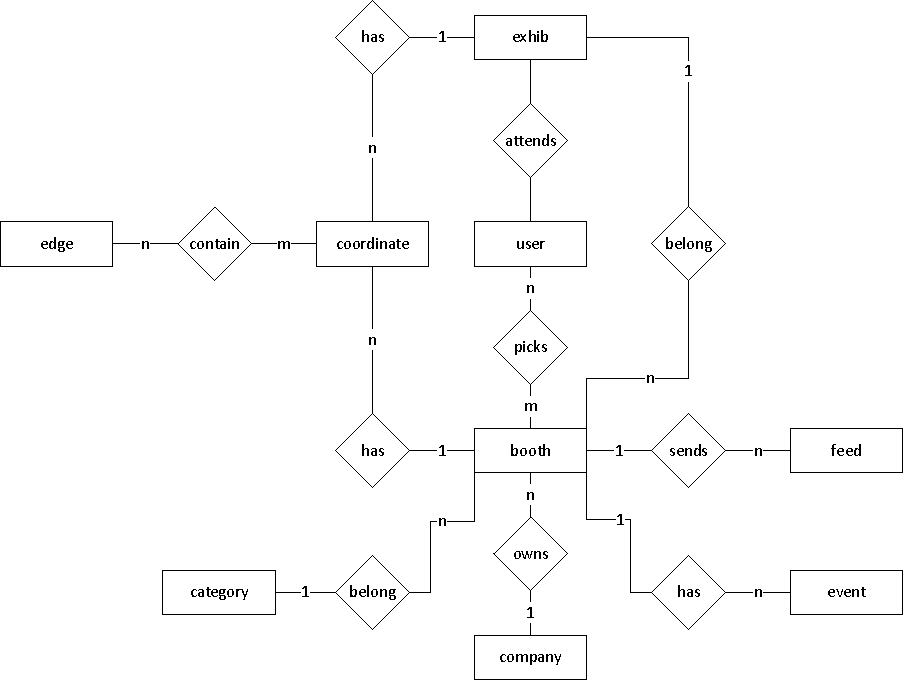
\includegraphics[page=1,width=1\linewidth]{img/sw7ERD.pdf}
\caption{Entity-relation diagram}
\label{fig:erd}
\end{figure}

%%% Local Variables: 
%%% mode: latex
%%% TeX-master: "../master"
%%% End: 
